%!TEX root = ../thesis.tex

\chapter{Verwandte Arbeiten} % (fold)
\label{cha:verwandte_arbeiten}

\begin{itemize}
    \item Verwendete Ansätze, Methoden und/oder Modelle (Sprachen, Entwurfsmethoden,Datenmodelle, Analysemethoden, Formalismen)
\end{itemize}

%------------------------------------------------------------------------------

\section{Semantic Interlinked Online Communities} % (fold)
\label{sec:verw_arbeiten_sioc}

Semantic Interlinked Online Communities\footnote{\url{http://sioc-project.org/}} (SIOC, ausgesprochen \enquote{schock}) ist ein Projekt, welches von Uldis Boj\=ars und John Breslin begonnen wurde um unterschiedliche, webbasierte Diskussionslattformen(Blog, Forum, Mailinglist,\dots) untereinander verbinden zu können \cite{Breslin2005}. Der Kern von SIOC besteht aus einer Ontologie, welche den Inhalt und die Struktur diese Plattformen in ein maschinenlesbares Format bringt und es erlaubt diese auf semantischer Ebene zu verbinden. Auch soll es so möglich sein Daten von einer Plattform zu einer Anderen zu transferieren und so einfacher Inhalte austauschen zu können. Als Basis für SIOC dient RDF, die Ontologie selber wurde in RDFS und OWL designt. Um nicht das Rad neu erfinden zu müssen greift SIOC auf schon bestehende und bewährte Ontologien zurück. Für die Abbildung von Beziehungen zwischen einzelnen Personen wird Friend of a Friend\footnote{\url{http://www.foaf-project.org/}} (FOAF) und für einige Inhaltliche- und Metadaten (Titel, Inhalt, Erstelldatum, \dots) Dublin Core Terms\footnote{http://dublincore.org/documents/dcmi-terms/} eingesetzt.



\begin{figure}[ht]
    \centering
    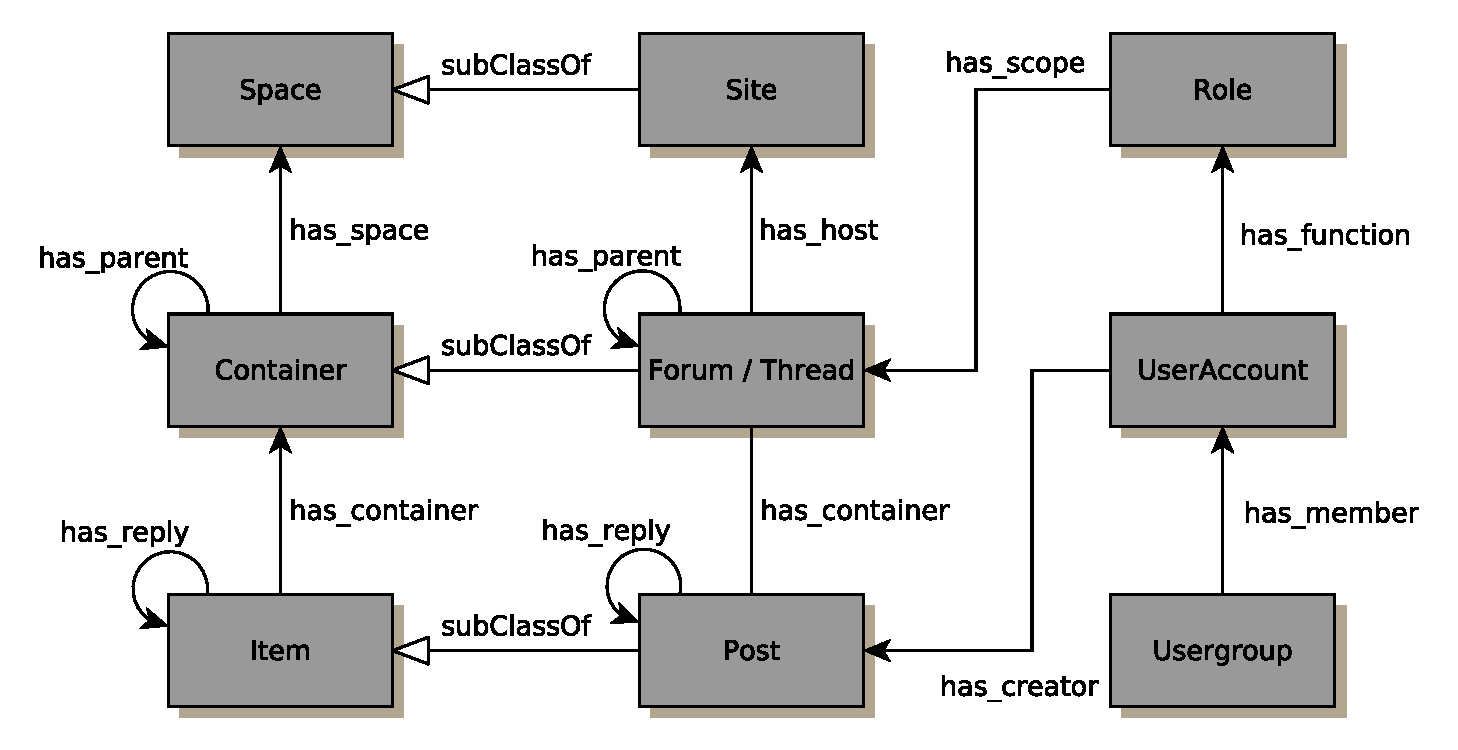
\includegraphics[
        width=\textwidth,
        keepaspectratio=true,
        clip=true]
        {assets/images/sioc_overview}
    \caption{Aufbau von SIOC (modifiziert) - Originalquelle: \cite{deri2013}}
    \label{fig:sioc_aufbau_diagramm}
\end{figure}


%------------------------------------------------------------------------------

\section{Reclaim Social} % (fold)
\label{sec:verw_arbeiten_reclaim_social}

Hat sich nicht jeder schon einmal vor den Rechner gesessen um, zum Beispiel, nach einen Bild gesucht das man irgendwann auf irgendeinem der unzähligen sozialen Netzwerke hochgeladen hat, einem aber partout nicht einfallen will wo? Wann und wo habe habe ich den Beitrag geschrieben, der perfekt zu meiner aktuellen Arbeit passen würde? Solche oder ähnliche Fragen wurden sicherlich schon mehrere Millionen mal von verschiedenen Menschen in der Welt des Internets gestellt. Wer hätte in so einen Fall nicht gerne alles was man über die letzten Jahre an verschiedenen Stellen im Netz geschrieben, hochgeladen oder als für ihn wichtig markiert hat zentral gespeichert um es durchsuchen zu können? Genau diesem Thema haben sich Sascha Lobo und Felix Schwenzel angenommen und auf der Netzkonferenz re:publica\footnote{\url{http://re-publica.de/}} 2013 ihr gestartetes Projekt \enquote{Reclaim Social} \cite{Schwenzel2013} vorgestellt.

\medskip

Ziel mit diesem Projektes soziale Medien aus allen möglichen Quellen auf seinen eigenen Blog zu spiegeln und so einen zentrale Anlaufstelle für seine eigenen Inhalte schaffen. Aufbauend auf der weit verbreiteten Blogsoftware \enquote{WordPress\footnote{\url{http://wordpress.org/}}} und der dafür vorhandenen Erweiterung \enquote{FeedWordPress}\footnote{\url{http://feedwordpress.radgeek.com/}}. Diese Kombination ermöglichst alle Internetseiten, welche einen RSS Feed\footnote{\url{http://www.rssboard.org/rss-specification}} anbieten, in die Datenbank von WordPress zu spiegeln. Das Problem hierbei besteht darin, dass einige sehr beliebte Internetseiten solche RSS Feeds nicht anbieten (\url{https://facebook.com}, \url{https://plus.google.com}) oder eingestellt haben (\url{https://twitter.com}). Für einige solcher Seiten wurden \enquote{proxy-scripte}\cite[Tecg Specs Details]{Schwenzel2013} implementiert, welche für diese einen RSS Feed emulieren. Zugleich können in den Feeds enthaltende Medien, wie Bilder und Videos(bisher nur als Referenz), heruntergeladen und in WordPress gespeichert werden. So ist es möglich alle gespiegelten Daten einfach zu durchsuchen oder nach bestimmten Kriterien zu filtern. Zusätzlich können alle Freunde, welche auch Reclaim Social einsetzen, in einen Kontaktliste eingetragen und so auch deren Inhalte eingebunden werden.

\medskip

Aktuell befindet sich dieses Projekt noch im Alpha Stadium und die Installation ist relativ kompliziert. Es ist aber geplant eine eigene Erweiterung für WordPress zu schreiben \enquote{he goal is to build just one Reclaim Social-plugin for any wordpress user}\cite[How Does It Work]{Schwenzel2013}




 

% chapter verwandte_arbeiten (end)